% !TeX root = ../main.tex

\chapter{绪论}

本章作为绪论主要介绍了神经辐射场中新视图合成加速问题的背景与意义,分析了目前相关技术与算法的发展现状以及相关系统存在的问题,阐述了解决该问题的必要性,然后总结了本文的主要工作与贡献,最后概述了本文的章节结构。

\section{研究背景与意义}
近年来,随着深度学习与计算机视觉的飞速发展,人类的生活愈来愈趋向智能化。在以前,人们必须通过行万里路来了解这个世界,但是现在,可以通过全景地图几乎全方位地去观察一个未知的地方,甚至是通过虚拟现实,增强现实等形式沉浸式地以任意的角度呈现出场景或者物体。新视图合成技术可以支持以上应用场景,可以通过已有的图像去合成新视角下的图像。

新视图合成任务\cite{chen1993view}作为计算机视觉和计算机图形学的交叉领域任务,有着极其广阔的应用前景,一直是学术界和工业界的热门研究问题。新视图合成任务具体是,通过给定的已知视角下观测到的图像,去合成新视角下的图像。图~\ref{fig:FreeViewSynthesis}给出了新视图合成任务的示意图。

\begin{figure}[tbhp]
    \centering
    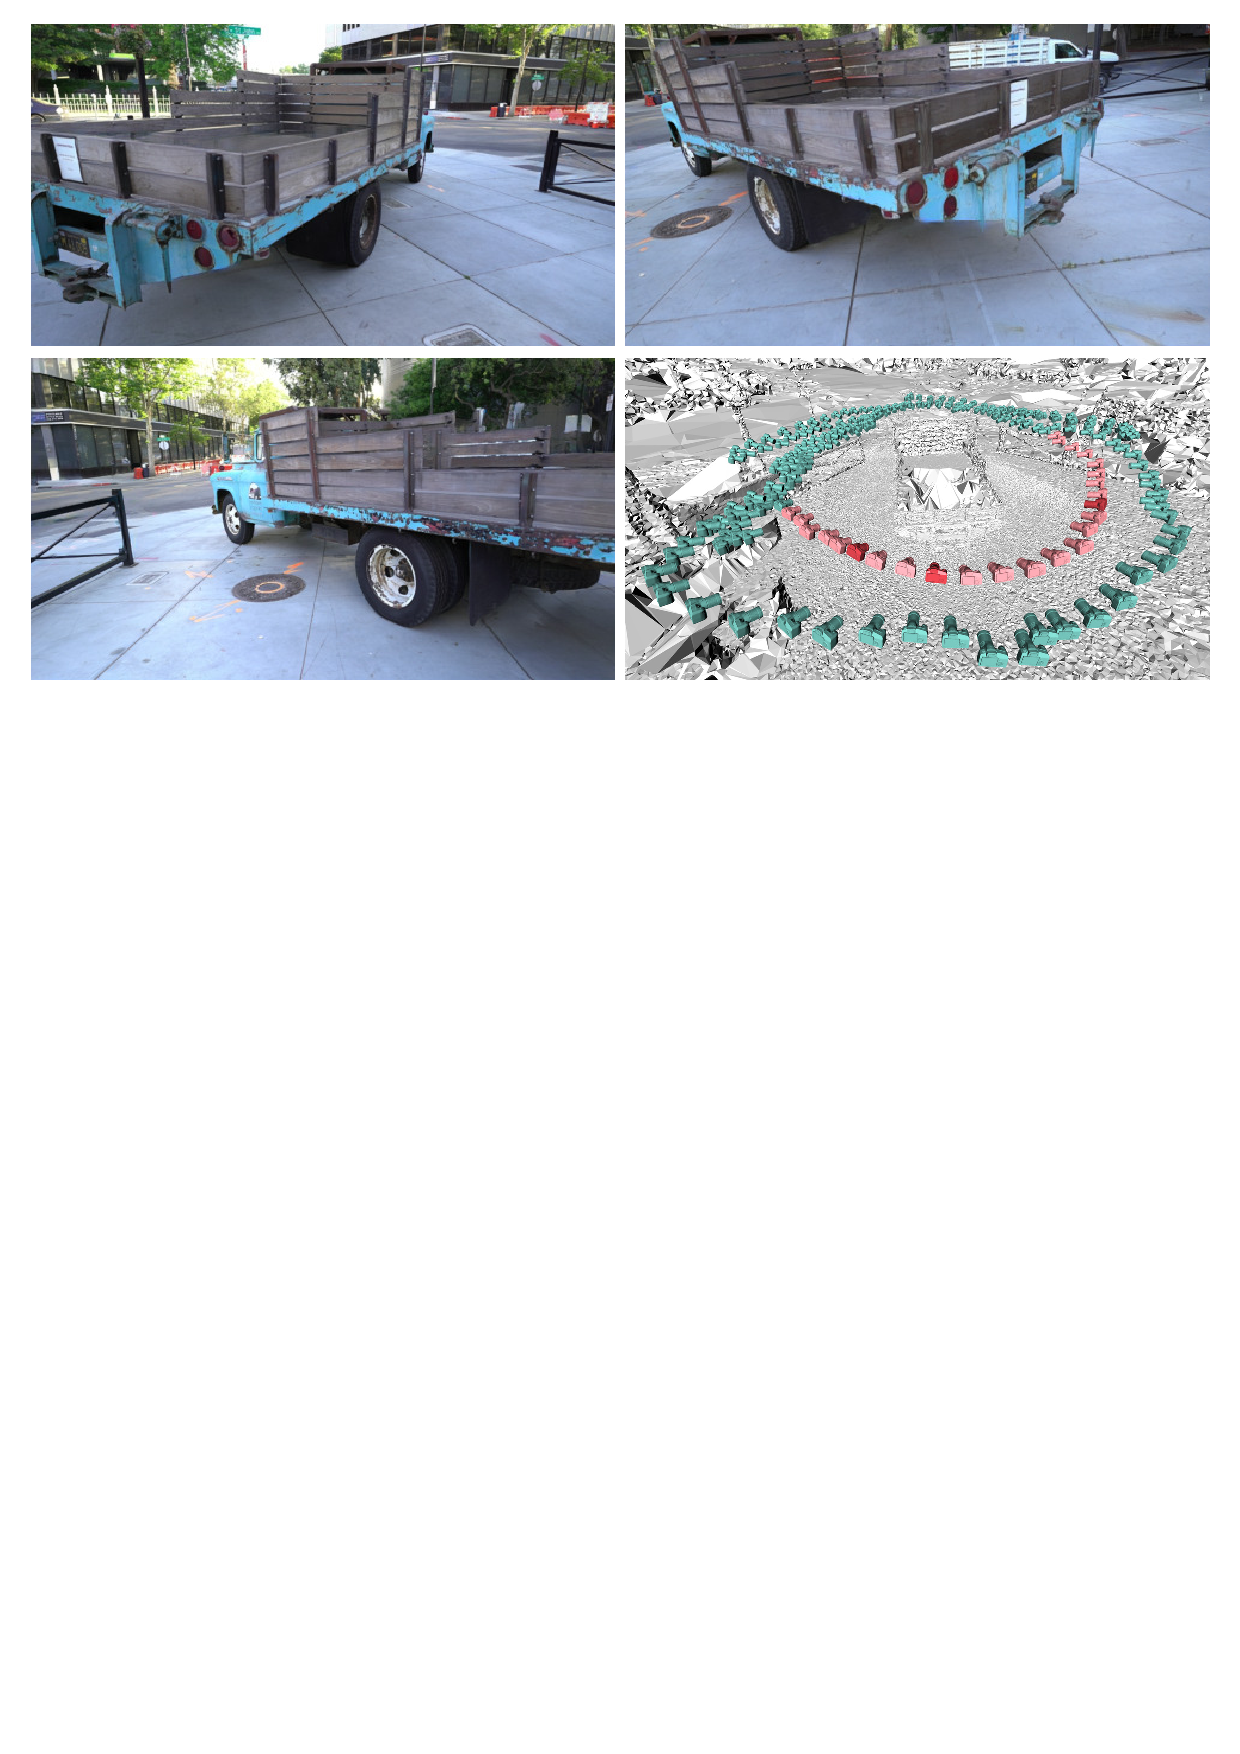
\includegraphics[width=0.95\textwidth]{figures/FreeViewSynthesis.pdf}
    \caption{新视图合成的示意图\cite{riegler2020free}。前三张图是合成的新视图,最后一张图阐明了绿色相机位姿下的图像作为输入,推理红色相机位姿的新视图}
    \label{fig:FreeViewSynthesis}
\end{figure}
\newpage

根据前期调研,新视图合成技术有着广泛的应用前景,市场需求庞大,急需可快速合成高质量新视图的系统。而在实际应用中,限于应用需求和经济成本等因素的考量,市场上的大多产品仍存在着许多问题,比如无法在任意角度合成高质量图像,另外渲染新视图的时间过长,这些都严重影响了用户体验。而本身,三维场景具有一定复杂性,市面上的很多软件在渲染之前需要进行复杂的三维建模,这很考验硬件的算力和内存。这些都增加了系统的实现难度。

具体地,现有的系统中存在以下一些问题:1) 当前市场上的三维渲染的软件难以根据稀疏视图,在任意视角下渲染出高质量的新视图;
2) 目前的三维渲染系统大都需要根据深度信息进行三维建模,这需要使用 RGBD 相机,对硬件设备要求较高;
3) 目前市场上还没有直接可应用的面向快速新视图合成的交互系统;4) 现有的新视图合成模型需要在空间内进行大量采样,计算时间成本较高,难以完成 PC 端的快速交互需求。

如果想要把新视图合成技术很好地应用在虚拟现实等技术上,那么必须能够在任意视角下合成几乎与真实场景相同的图像。这在合成场景下是可能实现的,但是在真实场景中,无法获得准确的相机位姿、光照条件难以建模等问题都限制了更好的体验,新视图合成仍面临着许多挑战。

% 主要挑战是通过给定稀疏的观测图像来推断场景的三维几何结构,以及对场景中遮挡和看不见的地方进行修补。在经典计算机视觉中,基于图像的渲染 (Image-based Rendering, IBR\cite{debevec1998efficient,kee2013exposing}) 方法通常依赖于基于优化的多视图立体 (Multi-View Stereo, MVS) 方法,以将重构场景的几何形状并将观测转到新视图的坐标系中。然而,如果只有少量观测图像可用,场景包含依赖视图的影响或者新视角下大部分没有被观测的图像覆盖到,那么 IBR 可能失效会导致出现鬼影或者空洞等效果。最近,随着深度学习的发展,基于深度学习的神经渲染方法\cite{tewari2020state}被提出,旨在合成更高质量的新视图。2020年,Mildenhall等人\cite{mildenhall2020nerf}提出了基于神经辐射场 (Neural Radiance Fields, NeRF) 的方法去合成新视图,这使得神经渲染一度成为最优秀的新视图合成方法。NeRF 基于给定的稀疏图像,仅使用较为简单的全连接网络去隐式表达场景信息,最后使用体绘制的方法合成新视图。NeRF 是目前新视图合成任务中的渲染效果最佳的方法,但是由于使用体绘制进行渲染,要求必须在空间内进行大规模采样,这一方面会带来巨大的时间开销,另一方面采样点的位置的准确性将决定了神经辐射场拟合的准确性。



经典的基于图像的渲染 (Image-based Rendering, IBR\cite{kee2013exposing}) 方法可以完成以上任务,IBR 通常依赖于基于优化的多视图立体 (Multi-View Stereo, MVS) 方法,以此重构场景的几何结构。然而,如果只有少量观测图像可用,场景包含依赖视图的影响或者新视角下大部分没有被观测的图像覆盖到,那么 IBR 可能失效会导致出现鬼影或者空洞等效果。此外该方法需要对三维场景进行精细的三维重建,这会带来极大的计算开销,因此传统的基于图像的渲染方法难以应用到实际场景中。随着深度学习的发展,基于深度学习的神经渲染方法开始在新视图合成任务上展现出其惊人的渲染效果。
2020年,Mildenhall等人\cite{mildenhall2020nerf}提出了基于神经辐射场 (Neural Radiance Fields, NeRF) 的方法去合成新视图,这使得神经渲染一度成为最优秀的新视图合成方法。NeRF 基于给定的稀疏图像,仅使用较为简单的全连接网络去隐式表达场景信息,最后使用体绘制的方法合成新视图。如果有一个系统能够使用基于 NeRF 的方法快速渲染出高质量的新视图,那么将极大地提升用户体验。因此,在这样的需求下,本文致力于将具有最佳渲染效果的 NeRF 技术设计并实现成完整的新视图合成系统,并在不损失精度的情况下对其渲染过程进行加速。

NeRF 是目前新视图合成任务中的渲染效果最佳的方法,但是由于使用体绘制进行渲染,要求必须在空间内进行大规模采样,这一方面会带来巨大的时间开销,另一方面采样点的位置的准确性将决定了神经辐射场拟合的准确性。

本文主要关注的是渲染时间长这一问题。NeRF 为了获取对渲染图象贡献较高的采样点,同时优化两个神经网络,使用 coarse 网络的输出去估计采样点的分布情况,然后基于此分布进行二次采样并通过 fine 网络预测的颜色和体密度进行数值积分计算出 2D 图像对应像素的 RGB 值,这带来了极大的时间开销。同时为了拟合更准确的神经辐射场,NeRF 使用了较深的神经网络,这也增加了推理新视图过程的时间成本。以上正是本文需要加速的地方。

在这样的背景下,本文研究了基于神经辐射场的新视图合成的相关技术,认为基于深度学习的神经渲染方法存在着提升空间,并对现有方法 NeRF 进行了优化,设计并训练了可以快速合成高质量新视图的神经渲染模型。渲染效果受数据集的影响,一般来说合成场景下质量会相对好些,因为真实场景下问题比较多,比如相机标定不严格、相机位姿估计不准,照片畸变严重,光照条件难以建模等等。

最终,本文结合 NeRF 的技术以及查询表缓存加速的相关技术实现了快速合成新视图的神经辐射场渲染具体方法,并设计和实现了一个快速新视图合成的系统,完成了 PC 客户端的相关应用。与现有产品相比,该系统可以基于给定的稀疏图像,快速渲染出任意新视角下的图像,提供几乎和 NeRF 质量相同的新视图。

本课题来自于PixTalks公司的实际应用需求。

\section{国内外研究现状}
% \subsection{新视图合成相关系统应用现状}
% 为了了解新视图合成相关系统的现状,本文对相关产品进行了调研。目前市面上暂无直接具有新视图合成功能的系统或软件,都是将新视图合成技术嵌入到系统或软件的内部。    

\subsection{基于图像的神经渲染方法研究现状}
在计算机图形和计算机视觉中,基于图像的渲染方法通常是依靠场景的一组二维图像来生成三维模型,然后渲染该场景的一些新视图。一般基于图像的渲染 (Image-based Rendering, IBR) 方法根据是否使用几何信息分成两类。几何信息用于将图像内容从捕获的图像重新投影到新的目标图像域。在目标图像域中,源图像的投影被混合以合成最终图像。这种简化的过程仅能为具有精确几何结构且具有捕获足够多视图的物体提供较为准确的结果。但是,由于依赖于视图的影响,以及不完善的几何信息或太少的源图像,可能会出现诸如重影,模糊,孔洞或接缝之类的伪影。

\begin{figure}[tbhp]
    \centering
    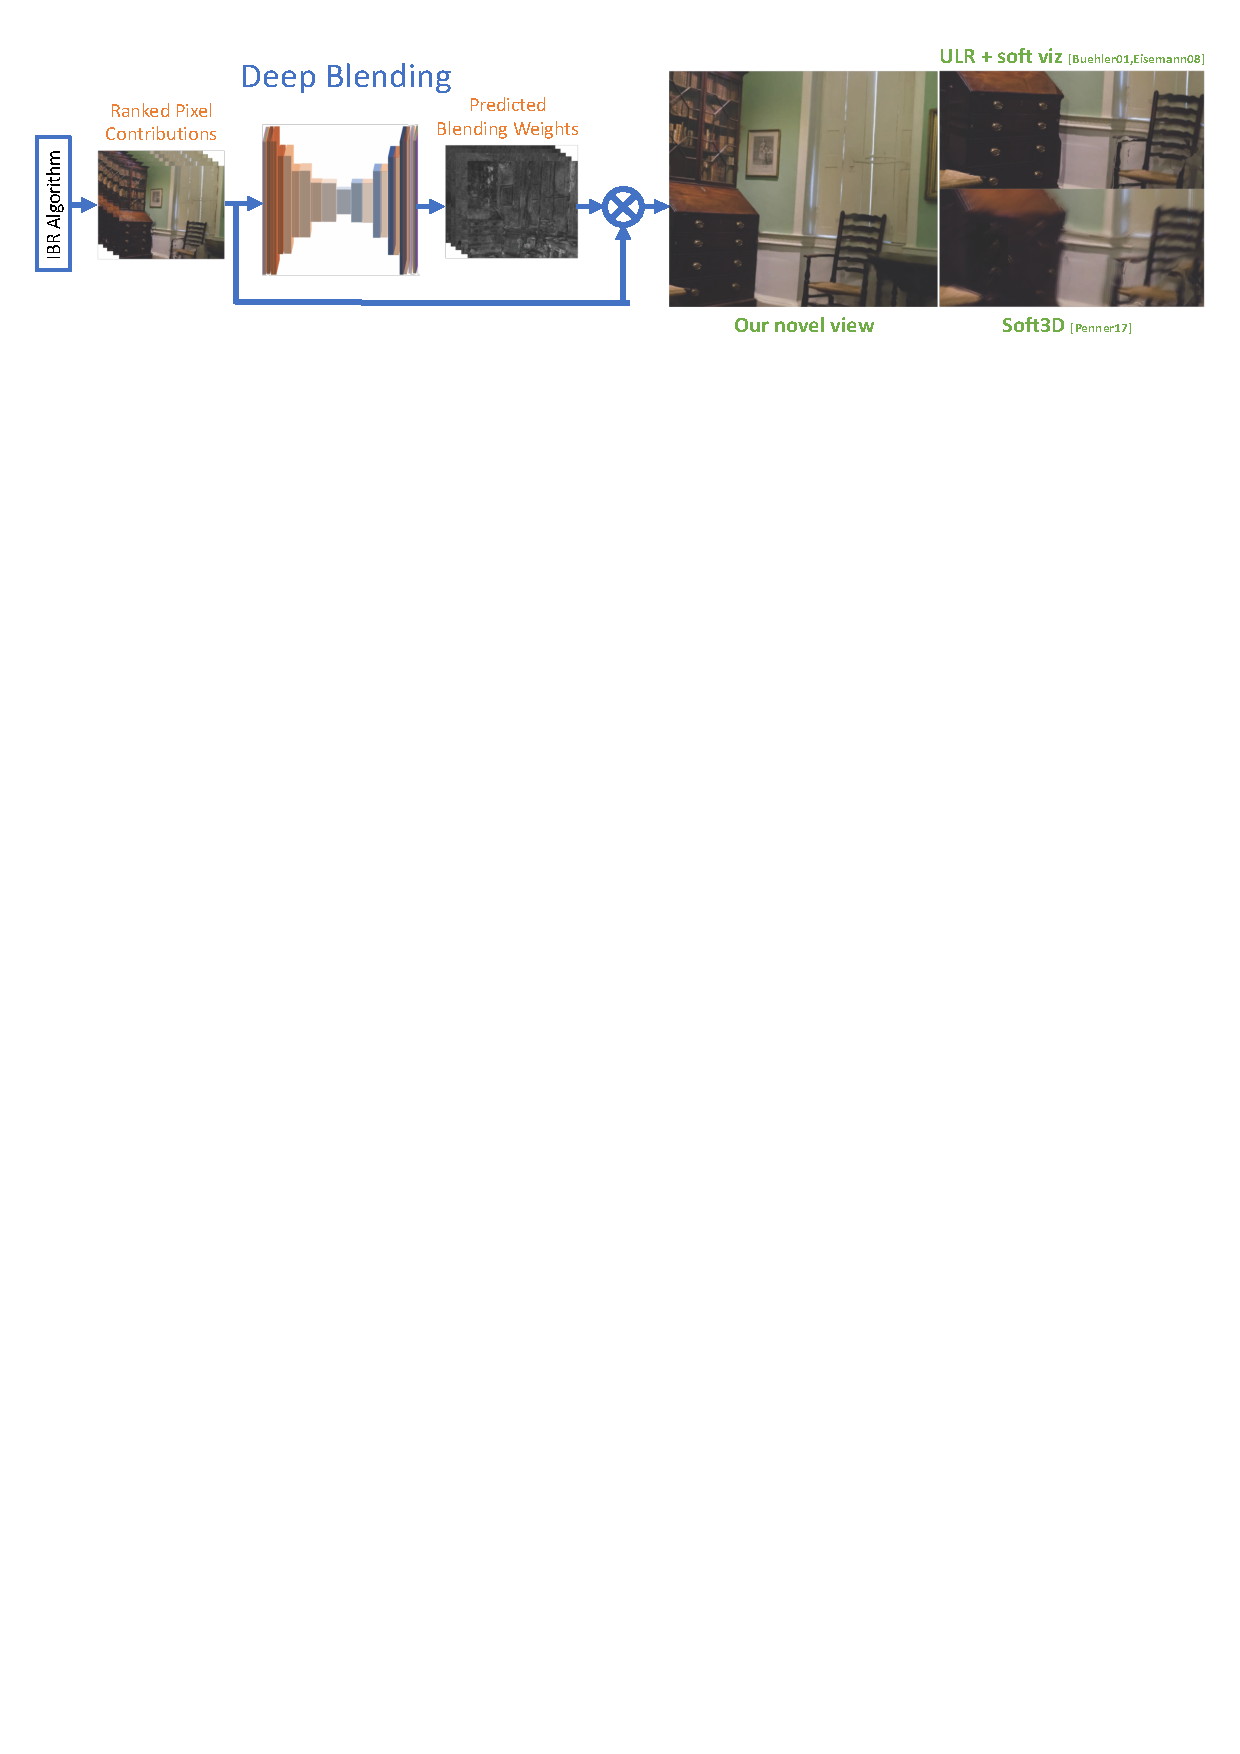
\includegraphics[width=0.95\textwidth]{figures/deepblending.pdf}
    \caption{DeepBlending\cite{hedman2018deep} 的框架结构,渲染效果较其他方法减少了伪影}
    \label{fig:deepblending}
\end{figure}

为了解决上述问题,将经典的基于图像渲染的方法与现如今最火的深度学习网络的结合成基于 IBR 的神经渲染方法,这极大地提升了 IBR 的渲染效果。DeepBlending\cite{hedman2018deep}提出了一种广义网络来预测投影源图像的混合权重,以便在目标图像空间进行合成。DeepBlending 在室内场景中显示了惊人的效果,比经典的 IBR 方法具有更少的混合伪影,具体见图~\ref{fig:deepblending}。事实上,DeepBlending 是将 COLMAP\cite{schonberger2016structure} 和商用软件 Reality Capture 进行了结合,以此获取更为精细的几何结构信息。COLMAP 基于块匹配的多视图几何算法进行稠密重建,这能够非常好地重建场景中的细节,但是与此同时在纹理信息缺失的地方也会出现空洞。Reality Capture 的结果相对完整,但是对于场景级别的区域重建的较差。因此,上述两种方法是互补的,将它们进行结合可以获得非较为准确的几何模型信息,DeepBlending 就是使用上述几何信息,借助神经网络来学习如何将不一致的观测图像信息进行混合,最终确实获得了非常惊艳的效果。但是,该方法过于依赖 COLMAP 三维重建出的几何信息,当几何信息较少时渲染质量会严重下降并伴随伪影。此外,精细的三维重建会带来非常大的计算开销,这在实际中难以使用。因此这种经典的基于 IBR 的方法无法满足本系统的速度和质量需求。

%其他方法如 NPBG\cite{aliev2019neural} 和 NPCR\cite{dai2020neural} 使用比 mesh 更容易获得的点云作为三维代理几何体。由于点云自身的稀疏性特征,很可能会出现不应该观测到的点出现在新视角下,这是著名的 bleeding 现象。为了解决 bleeding 现象问题,NPBG 使用多分辨率的方式,将不同分辨率的特征图输入到后端网络中。不过,多分辨率的策略虽然解决了 bleeding 的问题,但是得到了相对模糊的渲染结果。	

\subsection{基于 NeRF 的新视图合成研究现状}
类似 DeepSDF\cite{park2019deepsdf},NeRF\cite{mildenhall2020nerf}借助深度学习的隐式表达方法,将三维几何场景中的光照和几何信息隐式表达在神经网络参数中,最后利用立体渲染的方法进行渲染。NeRF 算是基于图像的神经渲染方法中最具代表的工作了。NeRF 本身不需要任何的显式的几何信息,仅使用真实场景的 RGB 图像作为监督信号,使用深度神经网络自动推理相关几何以及光照信息。NeRF 凭借着其网络简单,渲染效果惊艳的特性,备受学术界和工业界的关注。自从 NeRF 的出现,基于神经辐射场的新视图合成相关工作开始大量涌现。

NeRF++\cite{zhang2020nerf++} 首次指出 NeRF 具有形状光线的歧义性问题,即 NeRF 在一个场景下训练好的网络,其对应的空间表示可能是错的,但是仍能在训练集上渲染出正确的结果。

%\begin{figure}[tbhp]
%    \centering
%    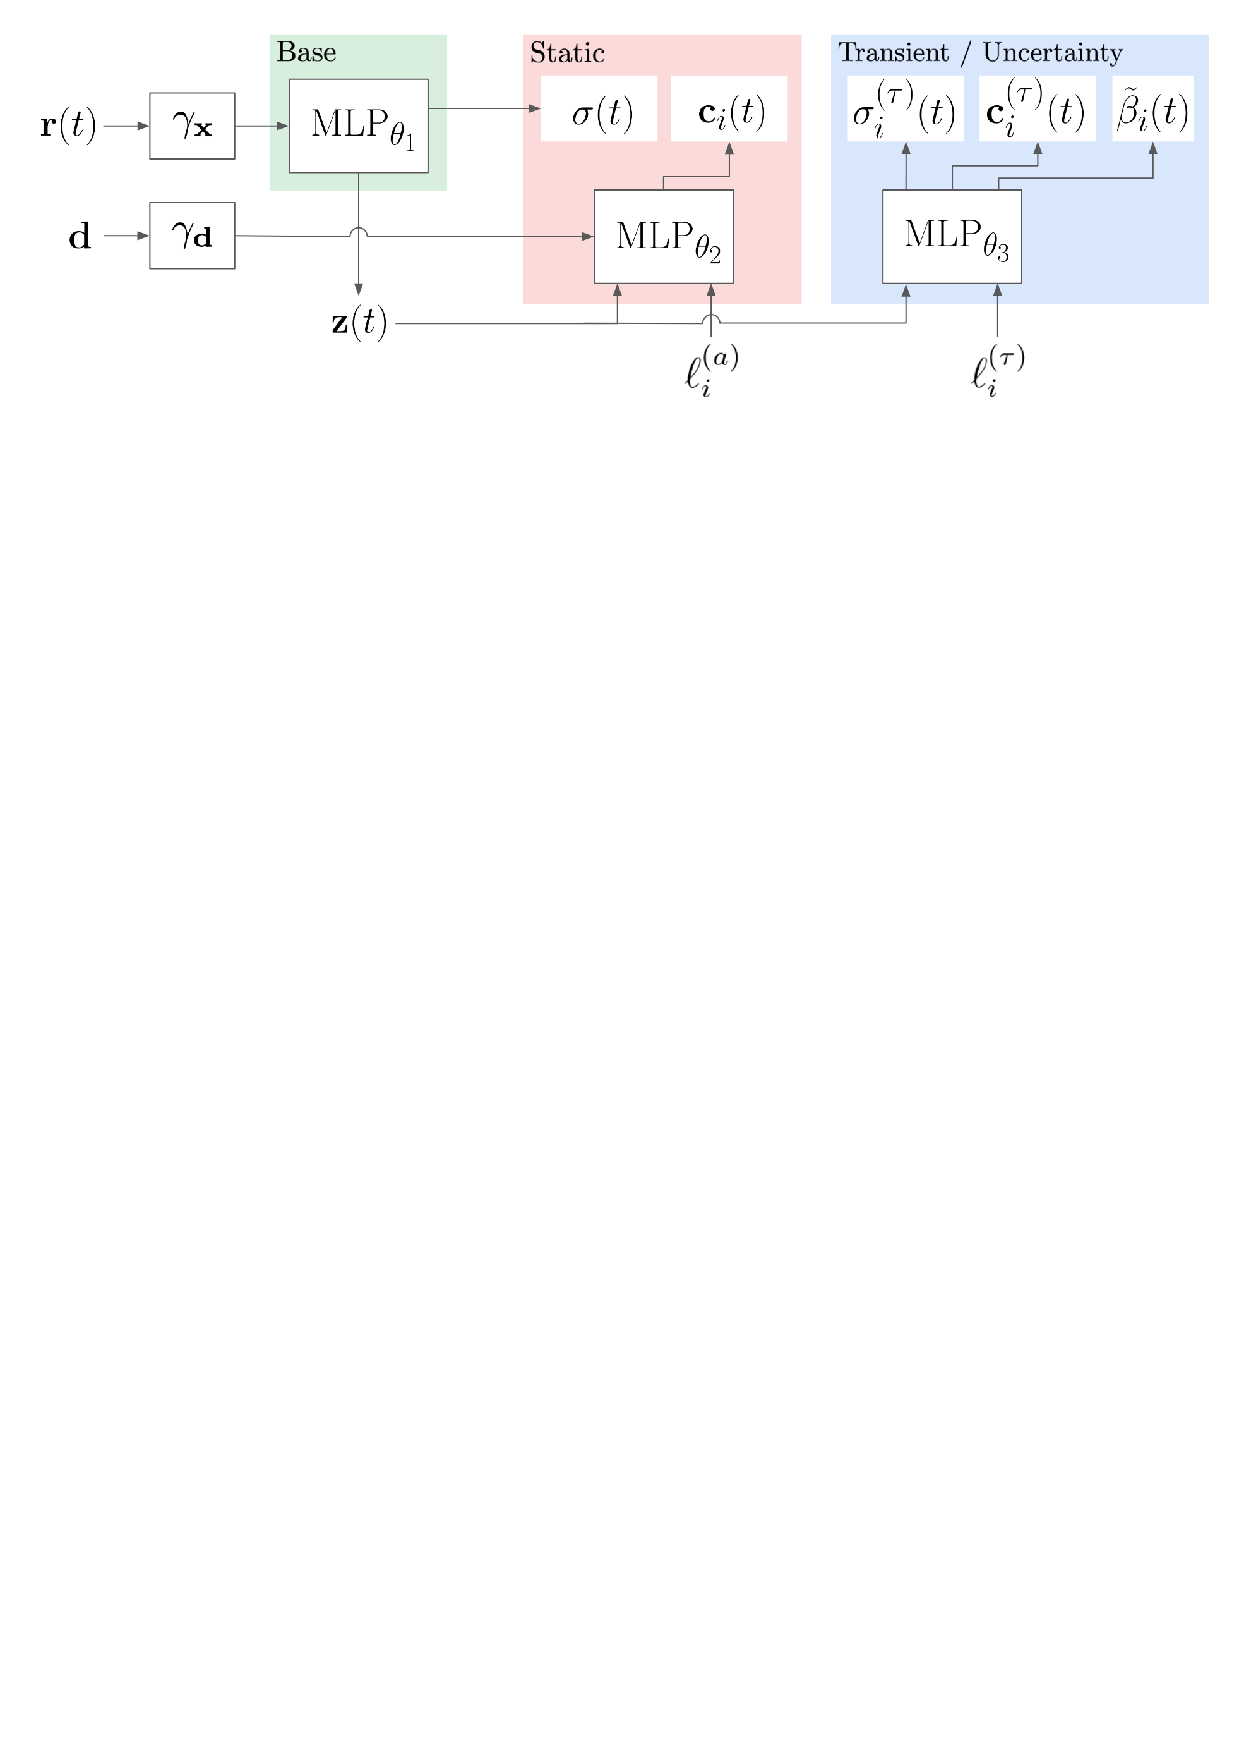
\includegraphics[width=0.95\textwidth]{figures/NeRF-W.pdf}
%    \caption{NeRF-W\cite{martin2020nerf}的网络框架示意图}
%    \label{fig:nerf-w}
%\end{figure}
%
%之后 NeRF-W\cite{martin2020nerf} (NeRF in the Wild) 对 NeRF 进行了另一种补充改进。由于 NeRF 假设输入的图像是由静态场景生成的图像,每张图所表示的场景具有相同的光照条件和几何结构,这在实际中是很难保证的。对于这个问题,如图~\ref{fig:nerf-w}所示,NeRF-W 给每张图片都预先编码了两个固定向量,分别是 $l_i^{\left(a\right)}, l_i^{\left(\tau\right)}$。其中,$l_i^{\left(a\right)}$ 是用来学习当前的光照条件,而 $l_i^{\left(\tau\right)}$ 是用来学习当前图像是否有动态物体遮挡,将这两个embedding 输入网络会输出一个不确定度。以上的做法让 NeRF-W 在真实场景下能够表现地更加鲁棒,在光照条件变化以及动态的场景下都取得了非常好的效果。

Yen-Chen等人\cite{yen2020inerf}基于位姿估计方法给 NeRF 提供了新的改进思路,推出了新工作 iNeRF。NeRF 在处理真是数据集的时候,位姿是通过COLMAP\cite{schonberger2016structure}进行计算的,然而这并不能获得绝对精准的位姿,也即送入网络的采样点是不准确的,那么也无法准确拟合真是场景的神经辐射场。如图~\ref{fig:inerf}所示的是 iNeRF 的网络框架,注意到,颜色的均方误差对坐标是可微的,而坐标对相机位姿也是可微的,因此,可以在训练神经辐射场的同时对位姿进行优化,具体是采用神经网络的反向传播算法进行优化的。此外,为了更有效地优化位姿,iNeRF 使用了 ROI 采样方式,即对感兴趣的区域进行采样优化,这样能显著缓解直接采样一张图片带来的内存开销大的问题。iNeRF 通过位姿矫正,最终在真实场景下显著提升了 NeRF 的渲染质量。不过,由于训练时每一张图都要单独优化位姿,而渲染时相机位姿仍然是不准确的,因此本系统暂不考虑位姿的问题。

\begin{figure}[tbhp]
    \centering
    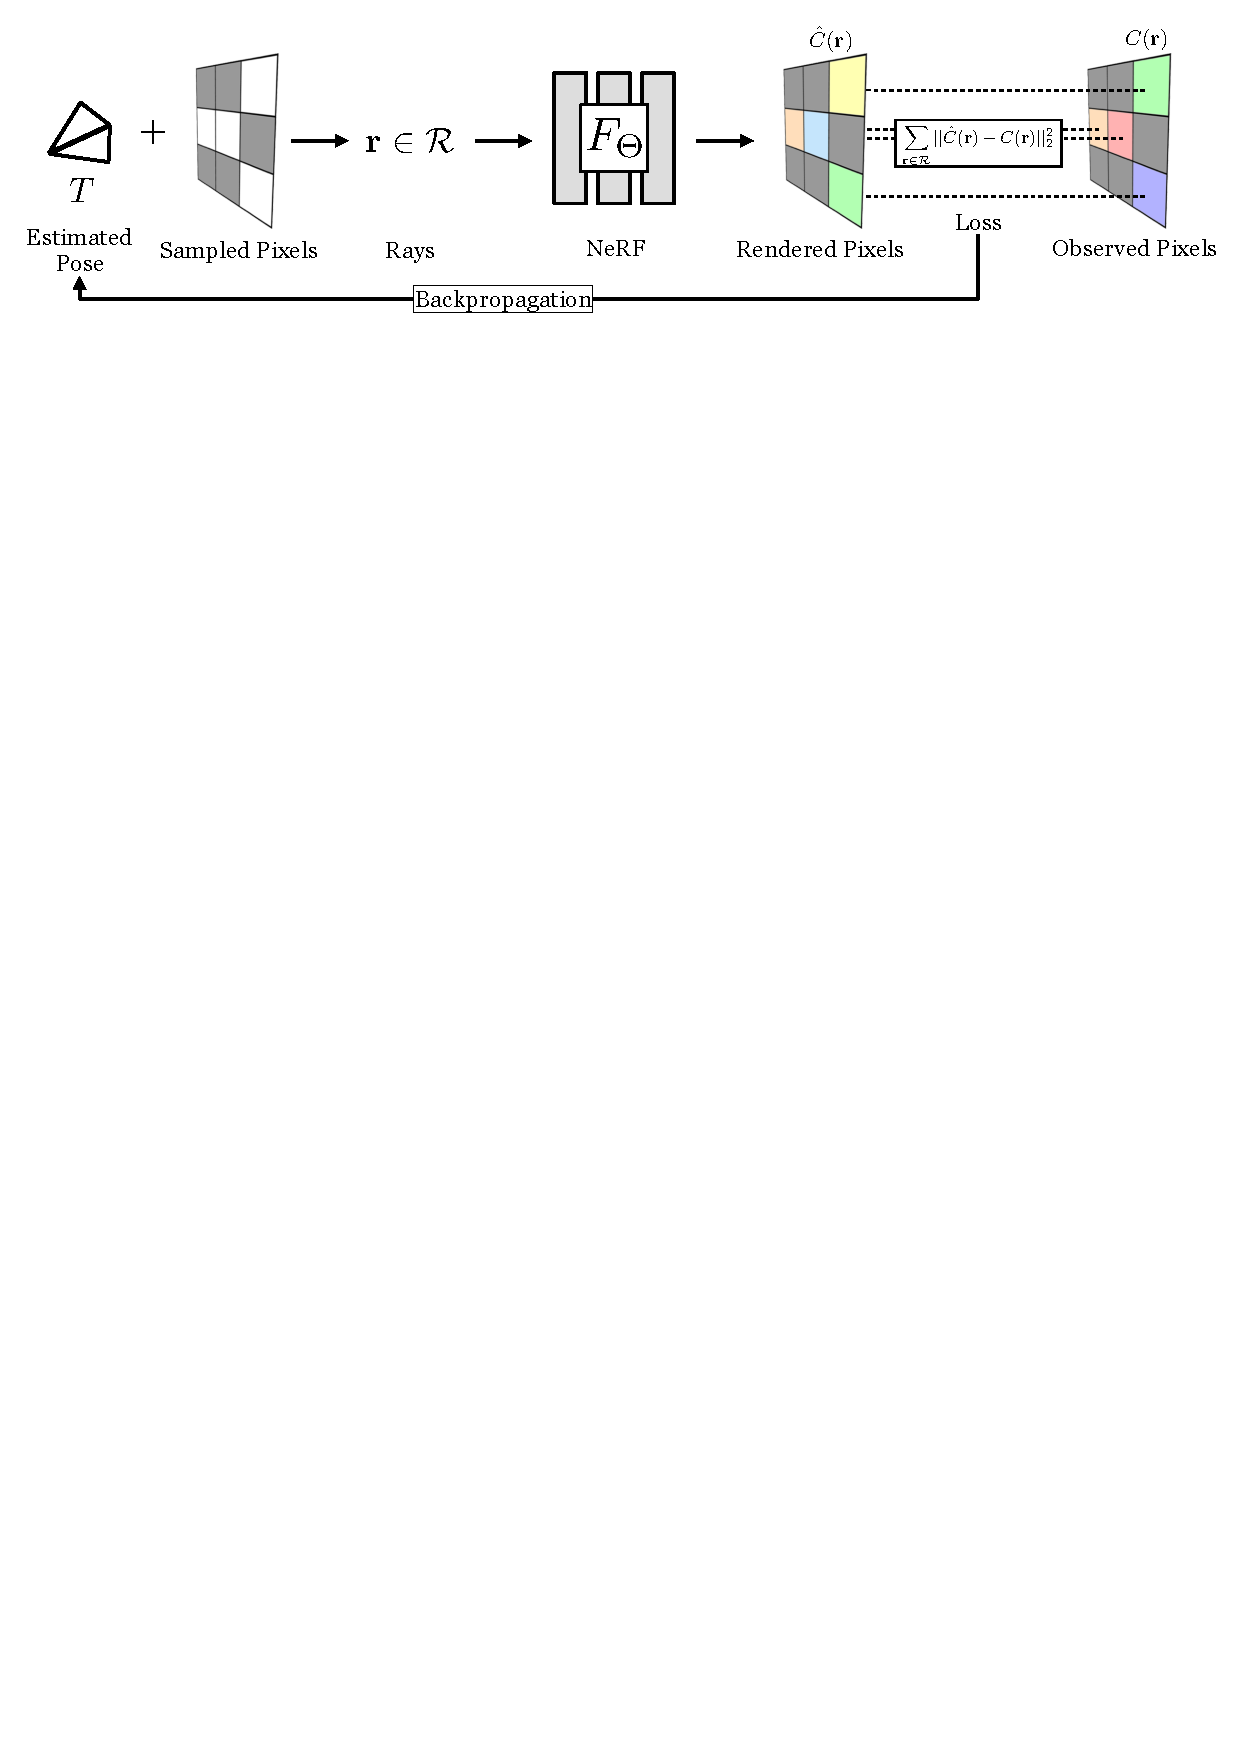
\includegraphics[width=0.95\textwidth]{figures/iNeRF.pdf}
    \caption{iNeRF\cite{yen2020inerf}的网络框架示意图}
    \label{fig:inerf}
\end{figure}

上述方法都还是基于多层感知机 (MLP, Multilayer Perceptron) 训练的。下面介绍一些对 NeRF 网络上进行的一些改进的工作。PixelNeRF\cite{yu2020pixelnerf} 使用卷积神经网络 (Convolutional Neural Networks, CNN) 提取的特征,仅需要少量图片作为输入就可以合成新视角下的图像,并有一定的泛化能力。GRF\cite{trevithick2020grf}使用 CNN 提取包含光线属性的特征,并使用 attention 机制将采样点在不同视角下的特征进行聚合,极大地提升了渲染质量。GRAF\cite{schwarz2020graf} 使用对抗生成网络 (Generative Adversarial Networks, GAN) 对 NeRF 进行改进,使之具有较强的泛化能力。但是,以上这些基于网络的改进方法都使得网络变得过于复杂,有些违背 NeRF 网络简洁的初衷,会使得训练和渲染的时间过长,这不能满足用户对于快速合成新视图的需求,几乎无法应用到实际的系统中。

\begin{figure}[htb]
	\centering
	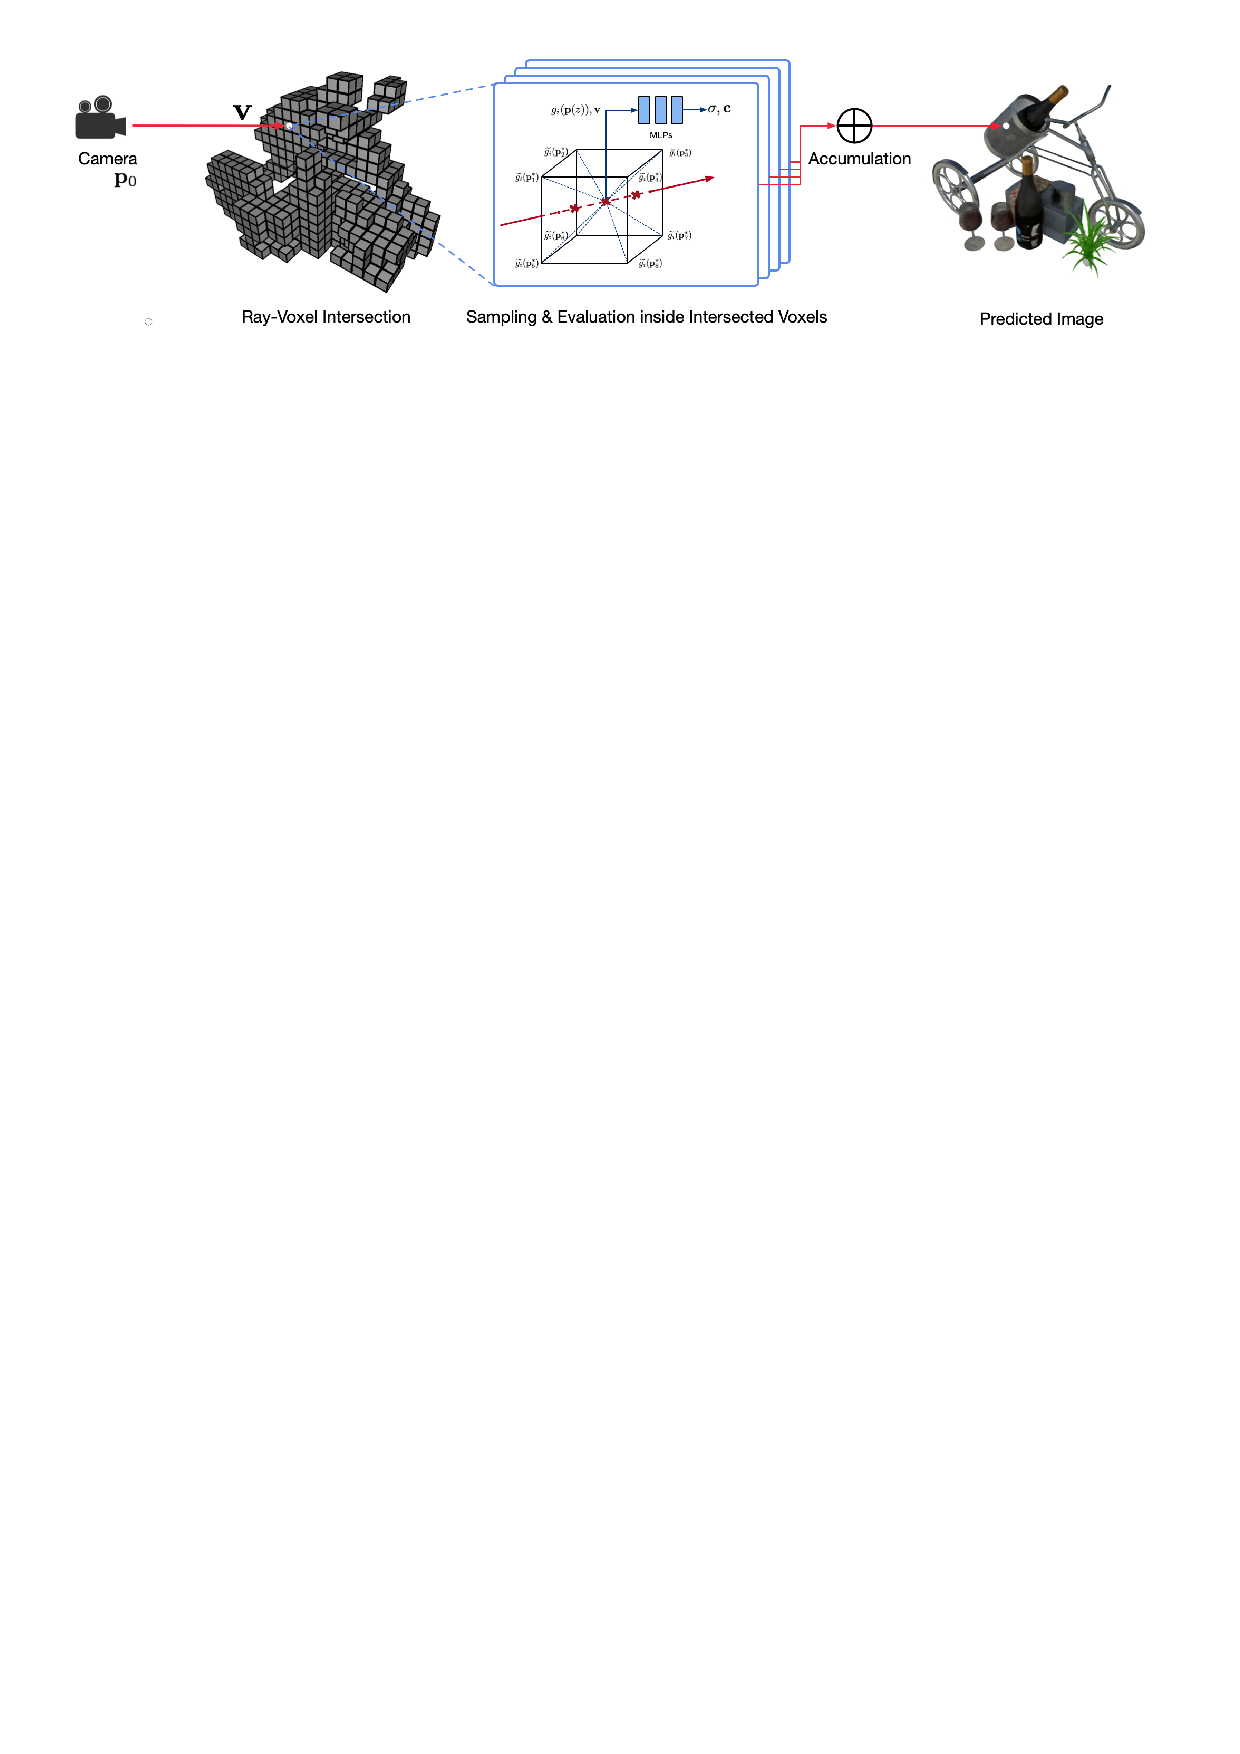
\includegraphics[width=0.95\textwidth]{figures/NSVF.pdf}
	\caption{NSVF\cite{liu2020neural}的网络框架示意图}
	\label{fig:nsvf}
\end{figure}

下面介绍一些基于 NeRF 的加速方法。由于 NeRF 需要在相机光线上进行大量的采样,这些采样点都要经过网络,而 NeRF 自身又使用了两个网络进行训练,因此 NeRF 的渲染是很慢的。如图~\ref{fig:nsvf},为了给 NeRF 加速,NSVF\cite{liu2020neural} 首先提出将空间划分为若干体素,使用自我裁剪的方法去掉体密度较小的体素,渲染的时候只需找到相机光线第一个穿过的体素,根据该体素八个顶点对应的特征进行插值编码并送入下游 MLP 预测出颜色和体密度,这避免了大量的采样计算,显著加速了新视图合成的过程。但是,NSVF 仅适用于简单的三维物体,在复杂的真实场景下渲染新视图的质量较差,甚至会出现鬼影,因此并不适合在本系统上使用。Lindell等人\cite{lindell2020autoint}提出了一种利用自动积分来进行渲染加速的方法 AutoInt。AutoInt 是通过隐式网络学习到闭式解求积分,从而取代了 NeRF 的数值积分,最终能为 NeRF 渲染过程加速10倍。不过,就 PSNR 来看,AutoInt 在合成数据集 Synthetic-NeRF 上平均比 NeRF 低\SI{5.4}{dB},这是一种重视加速但牺牲了很多质量的方法,并没有真正做到在不失精度的情况下对渲染进行加速。上述介绍的加速方法未能保证不损失精度情况下对 NeRF 进行加速,不符合本系统的需求,因此本文最终依旧使用最经典应用场景最丰富的 NeRF 技术并对其进行无精度损失的加速,最终完成整个快速新视图合成系统的构建。

\section{本文的主要工作与贡献}
% 基于神经辐射场的快速新视图合成系统的设计与实现中存在以下一些问题:1) 当前市场上的三维渲染的软件难以根据稀疏视图,在任意视角下渲染出高质量的新视图;
% 2) 目前的三维渲染系统大都需要根据深度信息进行三维建模,这需要使用 RGBD 相机,对硬件设备要求较高;
% 3) 目前市场上还没有直接可应用的面向快速新视图合成的交互系统;4) 现有的新视图合成模型需要在空间内进行大量采样,计算时间成本较高,难以完成 PC 端的交互需求。

本文将 NeRF 技术和查询表技术进行有机融合,设计并实现了基于神经辐射场的快速新视图合成系统。本文根据 NeRF 的特性提出了基于神经辐射场进行加速合成新视图的框架, 将其命名为 F-NeRF,通过 NeRF 预测的体密度有效地提取到物体的几何结构并缓存到查询表中,这一方面辅助了获取物体表面附近的对计算颜色有高贡献的采样点,另一方面减少了一个网络的开销,同时也简化了网络,这显著加速了渲染的过程。最后,本文将这 F-NeRF 这一方法有效地部署到 PC 端,将其实现成可交互的系统。

具体地,本文的主要工作与贡献如下:
\begin{enumerate}
    \item [1)] 本文基于 NeRF 预训练的网络预测的体密度信息构建出一个可以表征在物体内外的查询表结构,这一方面直接减少了查询表的尺寸,另一方面该查询表可以直接为空间内任意一点提供 NeRF 网络中间层的特征,这加快了神经网络的正向传播速度。
    \item [2)] 在缓存了上述查询表的基础上,本文改进了 NeRF 的采样过程,通过查询表找到光线上离物体表面最近的内点,使得 NeRF 可以仅在此点附近进行采样,从而不必再使用两个网络,这显著加速了 NeRF,同时这正是本文的核心贡献。
    \item [3)] 为了补偿查询表分辨率不够带来的精度损失,本文对 F-NeRF 进行再训练,将渲染质量提升到原 NeRF 的水平。
    \item [4)] 本文在公开的数据集上做了大量对比验证实验。在公开合成数据集 Synthetic-NeRF 和真实场景数据集 LLFF-NeRF 上,与 NeRF 相比,我们提出的 F-NeRF 方法分别加速 3.2 倍和 3.4倍。 
    \item [5)] 本文设计并实现了基于 NeRF 的快速新视图合成的系统,完成了相应的 PC 端的应用,并对该系统进行了详细的需求分析以及架构设计,最后将本文的方法实现并部署到了 PC 端,经过详细地测试,该系统满足实际应用需求。
\end{enumerate}

%1) 使用预训练的 NeRF 网络,构建出一个可以表征在物体内外的查询表,该查询表可以直接为空间内任意一点提供 NeRF 网络中间层的特征,这加快了神经网络的正向传播速度。
%2) 在缓存了上述查询表的基础上,本文改进了 NeRF 的采样过程,通过查询表找到光线上离物体表面最近的内点,使得 NeRF 可以仅在此点附近进行采样,从而不必再使用两个网络,这显著加速了 NeRF,同时这正是本文的核心贡献。3) 本文设计并实现了基于 NeRF 的快速新视图合成的系统,完成了相应的 PC 端的应用,并对该系统进行了详细的需求分析以及架构设计,最后将本文的方法实现并部署到了 PC 端,经过详细地测试,本文方法在合成场景和真实场景下的渲染速度对 NeRF 分别加速3.2倍和3.4倍,该系统满足实际应用需求。


\section{本文的组织结构}
本文的组织结构如下:

第一章是绪论,主要简述了本文研究内容的背景与意义,指出了本文研究问题的难点,并介绍了本文的主要研究工作和贡献,对国内外相关工作的研究现状的充分调研与分析,最后对本文的组织架构进行安排。

第二章是相关理论和技术,主要介绍了基于神经辐射场的快速新视图合成系统应用的核心技术和算法。

第三章是本文的主要工作,主要介绍了本文方法的问题定义,本文方法的预备工作,然后详述了我们改进的基于神经辐射场的新视图合成加速方法。

第四章是本文的实验部分。主要阐述了实验的基本设置,包含开发环境、数据集等等,其次介绍了实验实现的具体细节以及相关评测指标。最后通过大量对比实验来验证本文提出的方法的有效性,同时对一些实验结果进行分析和讨论。

第五章是系统设计与实现,主要介绍了将本文提出的 F-NeRF 方法应用到系统上的具体实现与架构设计。详细阐述了本系统的需求分析,包含主要用例分析,以及具体的系统架构设计,最后介绍了将本系统的模型移植到 C++ 代码上的方法。

第六章是系统的部署与展示,主要介绍了本文系统的开发与运行环境,对经典的测试用例进行了详尽的步骤说明,根据用例步骤完成了功能测试。从测试结果看,系统各项功能均能正常运行,合成新视图速度快且质量高。

第七章为总结和展望部分。总结了本文的主要工作和贡献,并指出工作中的不足之处。提出在未来研究过程中的可能的研究方向,并对可继续完善的方面进行展望。
% \begin{enumerate}
%     \item 主体部分包括引言 (前言),国内外文献综述,正文, 结语,参考文献。要求图表清晰,叙述流畅,章节有序,层次 分明。\\
%     引言 (前言)部分内容主要为本研究课题的学术背景及理论与实际意义;本研究课题的来源及主要研究内容;建立研究的线索与思路。

%     \item 文中的图、表、公式等,一律用阿拉伯数字按章顺序编号。如图 1-1、图2-2, 表 1-1、表 2-1,公式 (1-1) 等。图序及图名置于图的下方,居中排列;表序及表名置于表的上方,居中排列。详见第\ref{figures_tables}章的说明。

%     \item 参考文献
%     \begin{enumerate}
%         \item 参考文献为论文中所有引文、引用观点以及对论文有重要影响和启发的文献;
%         \item 参考文献按在论文中出现的先后依次排序;个别学科若通用该学科惯用的排序规范,可以例外;
%         \item 参考文献内容一般排列在论文末尾 (论文篇幅较大且引用文献较多的,可在每章末尾注出),序码与论文加注处对应;
%         \item 参考文献标注格式: 使用国标GB/T 7714-2015标准, 建议使用工具自动控制引文格式, 
%         以保证格式规范。
%         该\LaTeX{}模板已经对引文格式做了配置,
%         用户需要将所需参考文献的信息存在 \texttt{bib} 格式的文件\texttt{ref/refs.bib}中, 
%         通过 \verb|\cite{}|命令在恰当位置引用 (详见第\ref{citations}章的说明)。
%         \texttt{bib}文件可从文献管理工具导出或自己用 \texttt{JabRef} 等软件编辑。
%     \end{enumerate}

%     \item 注释:可以用 “脚注”或 “文后注”来标注引用著作中的一些观点和案例,但全文标注方式应统一。
% \end{enumerate}

